\section{Method}
To achieve the goal of this work, the creation of a fine-grained typicality manipulation method, a modular and sequential workflow needs to be designed, which can be seen in figure \ref{fig:method_overview}. A given real image first needs to be inverted using a GAN inversion model (section \ref{sec:method_gan_inversion}) and the corresponding latent code obtained. Using a latent space manipulation technique (section \ref{sec:manipulation}), multiple new latent codes can be found that should exhibit the desired attributes. These latent codes are passed through a custom generator model and thus turned into images for which the typicality scores can be calculated using the custom typicality assessors described in section \ref{sec:typicality_measures}.
\begin{figure}[ht!]
    \centering
    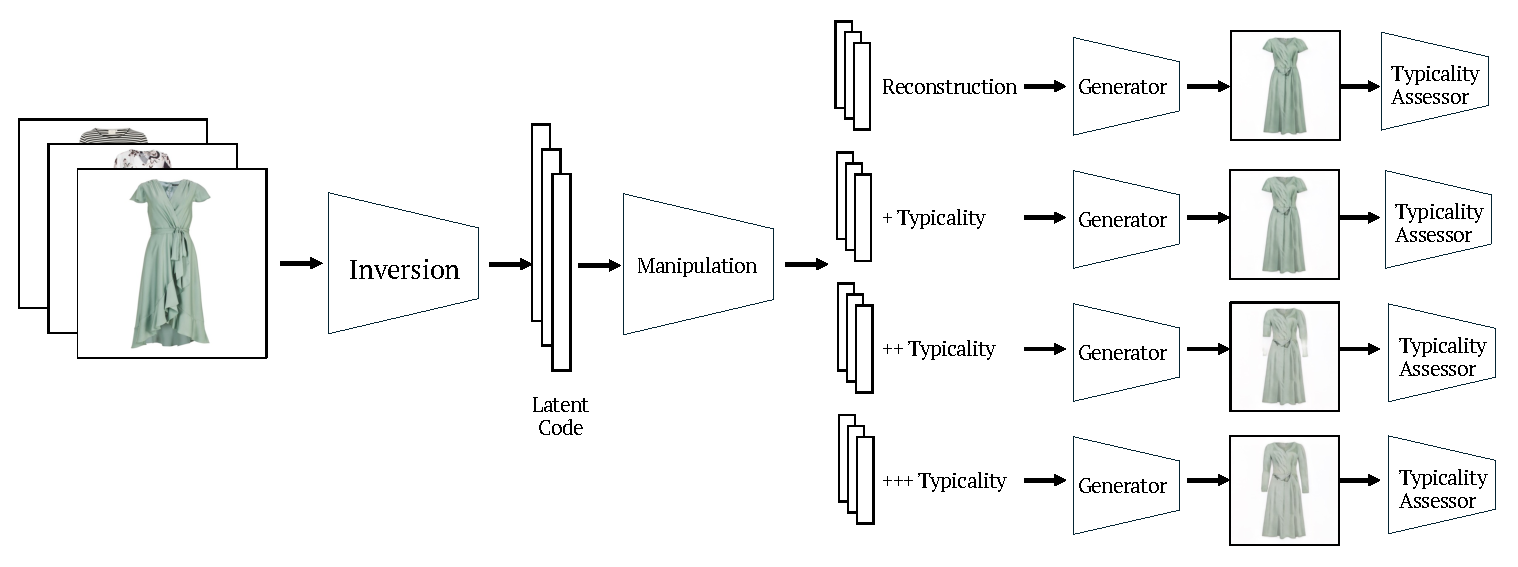
\includegraphics[width=1\linewidth]{Thesis/Method/assets/Method_Overview-cropped.pdf}
    \caption{Inference Workflow}
    \label{fig:method_overview}
\end{figure}
In practice, the order of training the models differs from this inference workflow (see figure \ref{fig:training_pipeline}). As a first step, a generator model needs to be trained which is capable of generating images similar to the distribution of the images one wants to manipulate. This generator model is used in the second step when building an inversion model that achieves good reconstruction and editing performance. As a third step, the typicality assessor is built using the reconstructions of the real images. In the last step, the manipulation model is trained based on the typicality scores and the latent codes from the inversion step.  In the following sections, I will explain the different steps of this process in more detail and explain the methods applied in this work.

\begin{figure}[ht!]
    \centering
    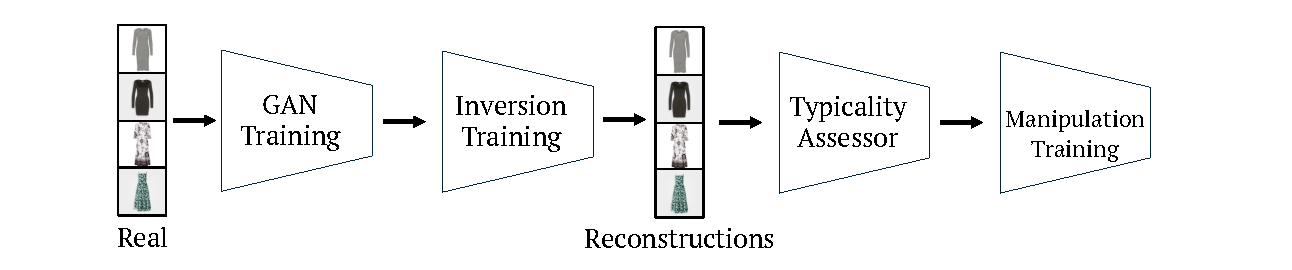
\includegraphics[width=1\linewidth]{Thesis/Method/assets/training_pipeline-cropped.pdf}
    \caption{Training Workflow}
    \label{fig:training_pipeline}
\end{figure}



%%%%%%%%%%%%%%%%%%%%%%%%%%%%%%%
% Dataset 
%%%%%%%%%%%%%%%%%%%%%%%%%%%%%%
\section{Dataset}
All models are trained on a newly created dataset of dresses from Zalando, one of the most popular online fashion retailers in Europe \citep[p.1]{freno2017practical}. The initial dataset consists of article information and image URLs of all publicly available dresses listed on the website "zalando.de" at the time of creation in March 2024. As a first pre-processing step, all articles that do not offer a standardized and centered packshot image of the dress are removed. Afterwards, all images are downloaded, squared in 1024x1024 resolution, and centered. Additionally, the article information is subset to attributes that offer good data completeness and non-noisy labels. The subset consists of the attributes "brand", "price", "category", "fabric", "fit", "neckline", "pattern", "collar", "length", "shape" and "sleeve length". These attributes are cleaned such that similar but small categories are grouped and categories with very few samples are recoded as missing to reduce the dimensionality of each attribute. Since there is no standardized color attribute, the color of each dress is obtained using a pre-trained CLIP model \citep[p.2]{radford2021learning} and a fixed list of 14 colors. The final dataset consists of 14,060 images with the corresponding article information from 643 unique brands. A random sample of images from the dataset can be seen in figure \ref{fig:random_samples}.

\begin{figure}[ht]
    \centering
    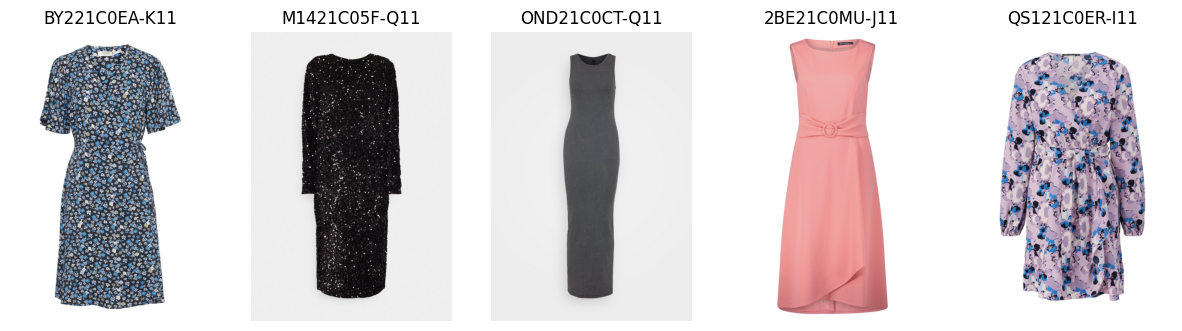
\includegraphics[width=1\linewidth]{Thesis/Dataset/random_sample.png}
    \caption{Random samples from the dataset}
    \label{fig:random_samples}
\end{figure}
% Generation 
%%%%%%%%%%%%%%%%%%%%%%%%%%%%%%
\subsection{Generation}
While multiple GAN-based architectures might be suitable, StyleGAN-based architectures have become the golden standard for image editing \citep[p.1]{bermano2022state}. This is mainly because they learn a highly disentangled and smooth latent space which allows for semantic attribute manipulation (see section \ref{sec:gans}). Within the family of StyleGAN-based architectures, StyleGAN2-Ada \citep{stylegan2ada} is chosen due to its remarkable capabilities to be trained on a small sample. Since the dataset acquired for training is limited by the availability of products on Zalando, training a traditional GAN model is not easily possible. Using StyleGAN2-Ada allows to train a high-fidelity generator even with a dataset of only 14k images.

\subsubsection{Training} \label{sec:sg2_training}
The StyleGAN2-Ada model used in this work has been trained for a resolution of 512x512 pixels per image using the "auto" configuration as defined in \cite{stylegan2ada} and additional x-flip augmentations to increase the dataset size. This configuration uses a reduced depth of the mapping network from 8 to 2 linear layers as this is sufficient according to the authors \citep[Appendix p.35]{stylegan2}. A transfer learning approach from the FFHQ-dataset \citep{stylegan1} is chosen since both datasets rely on centered images with non-relevant backgrounds. Using a pre-trained StyleGAN2-Ada model as the starting point speeds up the training process. The model has been trained for 26 hours on two NVIDIA Tesla V100 GPUs with 32GB VRAM. In total, 2000k images have been shown to the discriminator. Network snapshots have been saved every 40k images shown to the discriminator to later determine the best snapshot using the evaluation metrics described in section \ref{sec:gan_evaluation}.

\subsubsection{Evaluation}\label{sec:gan_evaluation}
The two most widely used GAN evaluation metrics are the Fr\'echet Inception Distance (FID) and the Inception Score (IS) \citep[p.2]{borji2022pros}. The IS \citep{salimans2016improved} evaluates the quality of generated images using ImegNet \citep{deng2009imagenet} predictions from an InceptionV3 \citep{szegedy2016rethinking} model. It combines the confidence of the conditional class predictions (indicating image quality) with the diversity of the predicted classes across the dataset (indicating image diversity). FID \citep{heusel2017gans} on the other hand calculates features of the real and generated datasets using intermediate layers of the same InceptionV3 \citep{szegedy2016rethinking} network and computes the Fr\'echet Inception Distance distance between them. \cite{heusel2017gans} define the FID using multivariate Gaussians over the extracted features as: 
$$\text{FID}(x, g) = \| \bs{\mu_x} - \bs{\mu_g} \|^2 + \text{Tr}\left( \bs{\Sigma_x} + \bs{\Sigma_g} - 2(\bs{\Sigma_x}  \bs{\Sigma_g})^{1/2} \right),$$
where $\bs{\mu_x}$, $\bs{\mu_g}$, $\bs{\Sigma_x} $ and $\bs{\Sigma_g}$ are the mean vectors and covariance matrices of the real and generated image distributions, respectively, and $\text{Tr}$ denotes the trace of a matrix. 

FID is consistent with human inspection and can detect intra-class mode collapse \citep[p.2]{borji2022pros}. As a drawback, for FID to be accurate and comparable, it needs to be calculated on a large and comparable number of samples. Hence, in all my experiments, I calculate the FID based on 50k generated images. As an alternative method, \cite{binkowski2018demystifying} proposed the Kernel Inception Distance (KID) which promises to be an unbiased version of the FID. In practice, there is a very high Spearman rank-order correlation between FID and KID \citep[p.3]{kurach2018gan}. While both the IS and the FID are single-score metrics that evaluate the quality and diversity of generations together, \cite{sajjadi2018assessing} propose improved formulations of precision and recall as GAN evaluation metrics. Recall estimates the fraction of the training set that the generator can reproduce while precision denotes the fraction of generated images that are realistic \citep[p.5]{kynkaanniemi2019improved}. Thus, when training a GAN, one aims for high precision and recall such that the generated images are as realistic as possible while also being as diverse as possible. Naturally, there is a trade-off between the two since a model that can create more diverse generations spans a much larger latent space, thus possibly allowing latent codes from ill-defined regions of this latent space that exhibit less realistic generations. To get a holistic assessment of the generation quality, I calculate all the above-mentioned evaluation metrics and select the best model snapshot based on a comprehensive analysis of the metrics.
%%%%%%%%%%%%%%%%%%%%%%%%%%%%%%
% Inversion 
%%%%%%%%%%%%%%%%%%%%%%%%%%%%%%
\subsection{Inversion}\label{sec:method_gan_inversion}
After a thorough literature review of available inversion methods (see section \ref{sec:gan_inversion}), a set of suitable methods was selected. The baseline model chosen is e4e \citep{tov2021designing} from the encoder-based models. Additionally, three hybrid models are tested: PTI \citep{roich2022pivotal}, ReStyle \citep{alaluf2021restyle}, and Hyperstyle \citep{alaluf2022hyperstyle}. Among these, PTI promises the best inversion performance but with a high inference time. To reduce inference time, ReStyle and Hyperstyle were selected as they promise similar results to PTI at a fraction of the time.

% After conducting a thorough literature research on available inversion methods (see section \ref{sec:gan_inversion}), a set of suitable methods has been selected. Since optimization-based methods have a prohibitively slow inference time and low editability performance \citep[p.3]{tov2021designing}, no pure optimization-based method has been selected. As a baseline inversion method, encoder4editing (e4e) \citep{tov2021designing} has been selected. This method promises high reconstruction quality while being specifically optimized to produce highly editable latent codes. Additionally, e4e is an encoder-based method and thus has a very fast inference time which allows to obtain latent codes for the complete dataset in a reasonable amount of time. Furthermore, many other inversion methods rely on e4e inversions as initial latent codes in their optimization. Using e4e, inversions into $\mathcal{W}^+$-space are obtained. The authors claim that there is a trade-off between distortion and editability when inverting into $\mathcal{W}$ or $\mathcal{W}^+$-space. While inversion into $\mathcal{W}^+$ leads to better reconstructions, it may come at the cost of editability \citep[p.5]{tov2021designing}. Encoder4editing for designed to specifically mitigate this, therefore in this work, only inversions into $\mathcal{W}^+$-space are used. From the domain of hybrid models, PTI \citep{roich2022pivotal} has been selected due to its proven state-of-the-art inversion performance \citep[p.1]{roich2022pivotal}. PTI builds upon e4e and uses its latent code as a starting point. It then pivots the generator weights such that the reconstruction quality increases. Since the latent code of the inversion is still the simple e4e inversion, it still lies in the editable region of the latent space, but thanks to the slightly changed generator, achieves much better reconstruction. Since the generator weights have to be optimized for each sample individually, inference time is very high. Therefore, two additional models have been tested which promise similar inversion performance at a fraction of the inference time. ReStyle \citep{alaluf2021restyle} and Hyperstyle \citep{alaluf2022hyperstyle} are models that again build upon e4e. ReStyle learns iterative refinement steps of the original e4e latent code by learning residual weights. Hyperstyle on the other hand builds upon ReStyle latent codes and additionally learns hyper-network weights for the convolutional filters of the generator. While this also changes the generator weights as in PTI, the hyper-network is learned during training and does not need to be optimized for every sample. Thus, inference time is drastically reduced.

\subsubsection{Training}
For training of the e4e model, the dataset has been randomly split into 90\% training samples and 10\% test samples. The model was trained with default parameters as defined in \cite{tov2021designing} and checkpoints were saved every 2000 steps.  In total, the model has been trained for 38 hours on one GPU. As can be seen in the loss curves for the overall loss, the LPIPS loss, and the L2 loss in figure \ref{fig:e4e_loss_curves}, the model has converged within this time. ReStyle and Hyperstyle have been trained with default parameters. ReStyle has initially been trained for 35 hours on one GPU but had not converged yet. Therefore it was trained for another 20 hours, totaling 55 hours of training time. Hyperstyle was trained for 40 hours and an additional 30 hours until convergence, totaling 70 hours of training time on one GPU. For all models, NVIDIA Tesla V100 GPUs with 32GB of VRAM were used.




\subsubsection{Evaluation}
Evaluating GAN inversion involves multiple dimensions. Generally, evaluation metrics can be grouped into three dimensions: Faithfulness (i.e. reconstruction quality), photorealism (i.e. perceptual quality),  and editability of the latent code \citep[p.3]{xia2022gan}. \\
Faithfulness measures the quality of the reconstruction, i.e. how closely the generated image from the inversion resembles the real image. One of the early measures proposed was Peak signal-to-noise ratio (PSNR). Many works additionally consider the Structural Similarity Index (SSIM) \citep{wang2004image} which measures the similarity using three key features: Luminance, Contrast, and Structure \cite[p.6]{wang2004image}. It has been shown that SSIM more closely correlates with human perception than PSNR \cite[p.19]{sheikh2006statistical}. For my evaluation, I use the advanced version of SSIM, the Multi Scale Structural Similarity Index Measures (MSSSIM) proposed by \cite{wang2003multiscale}.  Furthermore, multiple pixel-wise distances (e.g. mean squared error, mean absolute error) have been proposed. Since close reconstruction of input images is important in this work, the pixel-wise $\mathcal{L}_2$ distance will be used as an additional measure of faithfulness. \\
Measuring the perceptual quality of images (i.e. photorealism) against a reference dataset is described in chapter \ref{sec:gan_evaluation} in more detail. Many works rely on the same measures to evaluate the quality of the inversion process. I use the FID \citep{heusel2017gans} to measure how close the generated images from the inversions resemble the distribution of the real data. Furthermore, I use Learned Perceptual Image Patch Similarity (LPIPS) proposed by \cite{zhang2018unreasonable} which measures similarity between two images using features extracted from a VGG model \citep{simonyan2014very} trained on ImageNet \citep{deng2009imagenet}. \\
While the first two dimensions can be directly measured using multiple metrics, the editability of the latent code from an inversion method is not easily tested. Evaluating the editability involves yet another model, the editing technique. Thus, the evaluation of this dimension is very closely connected to the evaluation of the manipulation technique described in section \ref{sec:manipulation}. If the manipulation is not successful, it is difficult to find out whether the latent code itself is not editable or whether the manipulation method for the attribute does not work. As a qualitative measure for editing capabilities of inversions, \cite{zhu2020improved} propose to evaluate the quality of images generated from interpolating between two latent codes. They argue that an inversion is good if the interpolated images are of high quality \citep[p.10]{zhu2020improved}. In general, preserving the original identity during edits and only editing localized attributes is of high importance. \cite{alaluf2021only} and \cite{richardson2021encoding} use facial recognition networks as proposed in \citep{deng2019arcface} to assess identity preservation via cosine similarity of facial identity representations. For non-facial data, using this technique is challenging since training identity recognition networks for other domains is difficult \citep[p.13]{bermano2022state}. As \cite{tov2021designing} point out, all popular quantitative metrics to evaluate editing performance contradict each other and often the human judgment \citep[p.7]{tov2021designing}. \\
Given the difficulty of evaluating the editing capabilities of inversion methods, I focus on quantitative metrics for faithfulness and photorealism when comparing the different inversion methods. To assess the editing capabilities of the latent codes, I rely on interpolation experiments as proposed by \citep{zhu2020improved} and eventually on the results obtained from the downstream manipulation method.
\subsection{Typicality Measures}\label{sec:typicality_measures}
Measuring typicality, i.e. how "dressy" a dress looks like, is a central aspect of the overall workflow. Having a consistent typicality measure allows to create supervision needed in the training of the manipulation method. Furthermore, it allows to validate the success of the manipulation ex-post quantitatively. Based on work by \cite{landwehr2011gut}, typicality is measured based on the cosine similarity of a product's features (i.e. its embedding) to a morph of the features of all products. With $f(\cdot)$ being any embedding model, the d-dimensional embedding for dress $D_i$ is calculated as $\boldsymbol{v}_i = f(D_i)$. Furthermore, the morph of all dresses is 
$$\boldsymbol{m} = \frac{1}{n} \sum_{i=1}^{n}\boldsymbol{v}_i,$$
with $\boldsymbol{v}_i \in \mathbb{R}^d$ and $\boldsymbol{m} \in \mathbb{R}^d$. Finally, the typicality measure for dress $D_i$ is 
$$typicality = cosine\_similarity(\boldsymbol{v}_i, \boldsymbol{m}) = \frac{\boldsymbol{v}_i \cdot \boldsymbol{m}}{|\boldsymbol{v}_i||\boldsymbol{m}|}.$$
In the first step, as a simple embedding model the pre-trained Vision Transformer (ViT) DINOv2 \citep{oquab2023dinov2} is used. More specifically, the "Base" version is used with a patch size of 14, i.e. the "ViT-B/14" configuration. The resulting embeddings are 1x768 dimensional. The authors claim that the representations are task-agnostic and general-purpose \citep[p.1]{oquab2023dinov2} and thus can be used for typicality analysis. While this approach may overfit to non-essential attributes or use shortcuts, the second embedding model I use aims to produce more holistic and robust representations. It does so by forcing the embedding model to learn multiple sub-embeddings, one for each relevant attribute of the dress. Thus, the decision about which features or attributes are important to represent a dress is not exclusively taken by the model as in the pure DINOv2 case but is defined ex-ante based on domain knowledge. The model starts with the simple DINOv2 embeddings and passes them through some fully connected layers. Afterwards, the embedding is split up into k subspaces $a_1,a_2,...,a_k$ by individual classification heads $C_1,C_2,...,C_k$, one for each attribute. The attributes selected consist of \textit{Color, Fabric, Fit, Neckline, Pattern, Collar, Length, Shape} and \textit{Sleeve Length}. Since the goal is to achieve disentangled sub-embeddings, a distance correlation (dCor) loss is added to the model training, enforcing the reduction of shared information across sub-embeddings. The distance correlation proposed by \cite{muller2024disentangling} measures nonlinear dependencies between vectors of any dimension and has been used by the authors for disentangled representation learning. The dCor loss is defined as 
$$\mathcal{L}_{dCor} = \sum_{i \neq j} \text{dCor}(a_i, a_j),$$
with 
$$\text{dCor}(a_1, a_2) = \sqrt{\frac{\text{dCov}^2(a_1, a_2)}{(\text{dVar}^2(a_1) \text{dVar}^2(a_2))^{1/2}}}.$$
Details about calculating $\text{dCov}^2$ and $\text{dVar}^2$ can be found in the original paper \citep[p.5]{muller2024disentangling} and in the appendix in equation \ref{eq:dcor_formula} to \ref{eq:last_dcor_formula}. A schematic overview of the disentangled embeddings model can be found in figure \ref{fig:disentangling_embeddings}.

\begin{figure}[ht!]
    \centering
    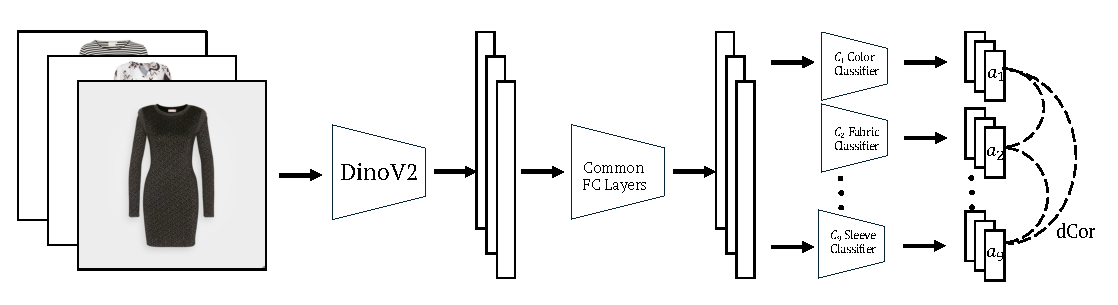
\includegraphics[width=1\linewidth]{Thesis/Method/assets/disentangling_embeddings-cropped.pdf}
    \caption[Disentangled Embeddings Model for Typicality]{Disentangled Embeddings Model for Typicality: \textit{Initial DINOv2 embeddings are divided into subspace embeddings $a_1,a_2,...,a_k$ by classifiers. Disentanglement is forced by a distance correlation loss between all sub-embeddings}}
    \label{fig:disentangling_embeddings}
\end{figure}

Each subspace embedding in this disentangled embedding model is 1x256 dimensional and thus the complete embedding, which is a concatenation of all subspace embeddings, has dimension 1x2304. Apart from the complete concatenation, I also construct embeddings that exclude one subspace at a time. This might be e.g. all subspace embeddings except the \textit{Color} subspace such that the model can calculate the typicality of a dress but does not take the \textit{Color} attribute of the dress into account.


It is important to note that both typicality measures are learned on the reconstructed images using the e4e inversion \citep{tov2021designing}. Thus, the embeddings for each dress, as well as the morphs, are calculated based on the respective reconstructions. Training the typicality measure on real images and using generated images at test time holds potential for problems. Although the reconstructions are very accurate, pixel values and low-level image features might differ between the generator outputs and the real image distribution, thus introducing possible mismatches in the typicality calculations.
%%%%%%%%%%%%%%%%%%%%%%%%%%%%%%
% Manipulation 
%%%%%%%%%%%%%%%%%%%%%%%%%%%%%%
\subsection{Manipulation}\label{sec:manipulation}
As mentioned before, I tested a linear (\textit{InterFaceGAN)} and a non-linear (\textit{StyleFlow}) approach, both from the family of supervised latent space manipulation techniques. Due to its low editing performance and prohibitively high computational cost, \textit{StyleFlow} has been disregarded after initial editing experiments on physical attributes like color or sleeve length of a dress. \textit{InterFaceGAN} on the other hand was used throughout all experiments in this work.

\subsubsection{InterFaceGAN}\label{sec:interfacegan}
The latent space of StyleGAN models is smoothly interpolable \citep[p.1]{stylegan1} and gradual changes in one direction in the latent space of a well-trained generator can result in gradual changes in a specific semantic attribute \citep[p.6]{bermano2022state}. \cite{shen2020interpreting} propose a simple, yet effective method of finding this direction in a method called \textit{InterFaceGAN}. The method is based on the assumption that for any binary semantic, a hyperplane in the latent space can be found that separates the two classes \citep[p.3]{shen2020interpreting}. Assuming a hyperplane with a unit normal vector $\mathbf{n} \in \mathbb{R}^d$, with $d$ being the dimension of the latent space, the "distance" of the latent representation of sample $\mathbf{z}$ to the hyperplane can be defined as 
\[d(\mathbf{n, z}) = \mathbf{n}^T\mathbf{z}.\]
If one moves towards and across the hyperplane in the latent space, the sign of the distance changes, and thus the semantic attribute in the generated image should have changed to the opposite class \citep[p.3]{shen2020interpreting}. 

\begin{wrapfigure}{r}{6cm}
    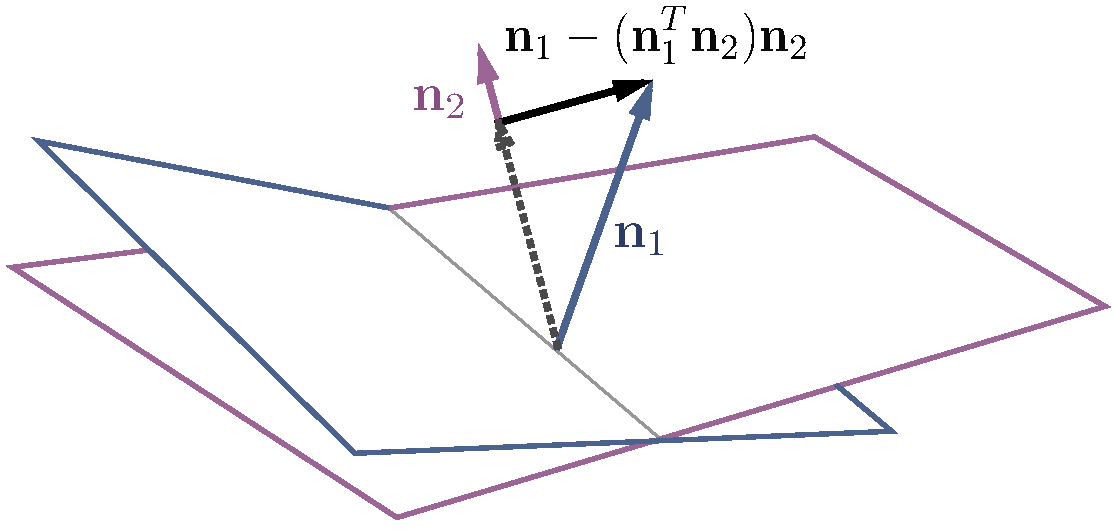
\includegraphics[width=6cm]{Thesis/Method/assets/subspace_projection.pdf}
    \caption[Conditional manipulation via subspace projection]{Conditional manipulation via subspace projection - taken from \cite{shen2020interpreting}, p.4}
    \label{fig:subspace_projection}
\end{wrapfigure} 

While this is straightforward for a single binary attribute, often multiple semantics are present and might not be independent of each other, although the latent space of StyleGAN models already enforces some degree of disentanglement (see section \ref{sec:gans}). In the case of $m$ semantics, $m$ separation boundaries $\mathbf{N} = [\mathbf{n_1, ..., n_m}]$ can be found. To disentangle them, $\{\mathbf{n_1, ..., n_m}\}$ need to be orthogonal to each other \citep[p.4]{shen2020interpreting}. In practice, conditional manipulation, i.e. editing one semantic without affecting any other semantic, can be performed using projection. As illustrated in figure \ref{fig:subspace_projection}, if one wants to manipulate the semantic connected with the hyperplane $\mathbf{n_1}$ without affecting the semantic connected with $\mathbf{n_2}$, the projection of  $\mathbf{n_1}$ onto $\mathbf{n_2}$ is subtracted from $\mathbf{n_1}$. Thus, the conditional manipulation direction is
$$\mathbf{n_{cond}} = \mathbf{n_1} - (\mathbf{n_1}^T\mathbf{n_2})\mathbf{n_2}.$$
For the semantic editing, the authors apply a simple linear manipulation of the latent space in the positive or negative direction of the unit normal vector $\mathbf{n}$ of the separation boundary. Thus the manipulated latent representation is defined as
$$\mathbf{z}_{edit} = \mathbf{z} + \alpha\mathbf{n},$$
with the synthesis being more positive on the semantic for $\alpha >0$ and more negative with $\alpha <0$ \citep[p.4]{shen2020interpreting}.

Since \textit{InterFaceGAN} is a supervised approach, either labels for the semantics or classifier scores need to be available. If there are labels available, those can directly be used to find a hyperplane that separates the latent space based on these labels. If only classifier scores are available, the authors propose to use the samples with the highest and lowest scores and assign binary labels. The hyperplane is then found by training a simple linear classifier on the latent representations. In this case, a linear Support Vector Machine (SVM) is trained. Linear SVMs learn a decision boundary which acts as the separation boundary in latent space that is used by InterFaceGAN.

\subsubsection{Training}\label{sec:interfacegan_training}

To make the \textit{InterFaceGAN} approach usable for this work, some implementation details needed to be adapted. While the authors used the 512-dimensional $\mathcal{Z}$-space of StyleGAN, I used the 16x512-dimensional $\mathcal{W^+}$-space. Thus, finding a hyperplane in this higher dimensional space is not as straightforward as in $\mathcal{Z}$. To tackle this problem, one could either flatten the latent representation in $\mathcal{W^+}$-space by concatenating all 16 dimensions along one dimension or learn 16 separate hyperplanes, one for each of the dimensions. The latter results in individual manipulations in each of the 16 dimensions. As explained in section \ref{sec:gans}, the various dimensions of $\mathcal{W}$ and $\mathcal{W^+}$ are injected at different levels of the synthesis process and allow targeted variations at different scopes of the image. Thus, learning isolated separation boundaries allows to apply targeted manipulation in the specific semantic only at a certain coarseness level of the generation process. On the other hand, learning one separation boundary from the complete latent representation allows the linear classifier to consider all features at all levels at the same time when finding the manipulation direction. Both approaches have been implemented and tested and the results are very similar. Since the isolated boundaries approach requires another step of selecting the dimensions to consider in the manipulation, the method of flattening the latent space has been selected as the final approach, thus simplifying the process without sacrificing editing performance. \\
When constructing the training data for the typicality scores, I closely follow the authors of \textit{InterFaceGAN} by using only the top $n$ and bottom $n$ scores in the classifier training. The idea is to create two distinct classes that can be clearly separated and that exhibit strong attributes of the two classes, i.e. high and low typicality. The boundaries have been computed using values of $n=1000$, $n=2000$, and $n=3000$. Finally, the separation accuracy on a separate validation set has been computed and the boundary with the best accuracy was selected as the final manipulation direction. \\
Another difference in the \textit{InterFaceGAN} implementation between this work and the original approach is the nature of the semantics. While the authors could show that the approach works well on naturally binary attributes like gender or the presence of glasses in facial images, or ordinal features like the age of a person, the labels present in the dresses dataset are different. Physical attributes like color or sleeve length, which are used as conditioning factors in the typicality manipulation, are nominal and have high cardinality. For those attributes, $\frac{n!}{2!(n-2)!}$ hyperplanes are calculated with $n$ being the number of unique values an attribute has. Therefore, there are hyperplanes for each combination of binary directions in the feature space. Defining one attribute value as positive while assigning all the others to the negative class (one-vs-rest) leads to multiple problems. First of all, the linear classification problem becomes extremely imbalanced. Furthermore, according to \cite{yang2021discovering} that set of negative samples provides ambiguous or even misleading guidance to the linear classifier, resulting in entangled semantics and incorrect manipulation directions \citep[p.1]{yang2021discovering}. When choosing a specific boundary as the conditional boundary, the set of boundaries to choose from is restricted to those that cover the real attribute value. So if the conditioning is on the color attribute and the dress is blue, all boundaries that include "blue" together with any other color are candidates. Out of the candidates, the boundary that has the best accuracy on the validation set during the classifier training is chosen. To visually validate the quality of these physical attribute boundaries, some preliminary manipulation tests using physical attributes have been run. The results of these experiments can be found in the appendix in figure \ref{fig:physical_attributes_manipulation}. Furthermore, descriptive statistics for the multiple separation performances of the physical attributes can be found in table \ref{tab:physical_summary_stats} in the appendix.




